%%%%%%%%%%%%%%%%%%%%%%%%%%%%%%%%%%%%%%%%%
% Projet de programmation
%
% Author:
% Julien Colot
%
%%%%%%%%%%%%%%%%%%%%%%%%%%%%%%%%%%%%%%%%%

%----------------------------------------------------------------------------------------
%	PACKAGES AND OTHER DOCUMENT CONFIGURATIONS
%----------------------------------------------------------------------------------------

\documentclass{article}

\usepackage{fancyhdr} % Required for custom headers
\usepackage{lastpage} % Required to determine the last page for the footer
\usepackage{extramarks} % Required for headers and footers
\usepackage[usenames,dvipsnames]{color} % Required for custom colors
\usepackage{graphicx} % Required to insert images
\usepackage{listings} % Required for insertion of code
\usepackage{courier} % Required for the courier font
\usepackage{tikz}
\usepackage{listings}
\usepackage{color}
\usepackage{subfig}
\usepackage{cite}


\usetikzlibrary{calc}
\usetikzlibrary{matrix,backgrounds}
\usetikzlibrary{decorations.pathreplacing}

%colors definitions
\definecolor{myblue}{RGB}{165,168,255}
\definecolor{mypink}{RGB}{255,179,231}
\definecolor{dkgreen}{rgb}{0,0.6,0}
\definecolor{gray}{rgb}{0.5,0.5,0.5}
\definecolor{mauve}{rgb}{0.58,0,0.82}

% Marges
\topmargin=-0.45in
\evensidemargin=0in
\oddsidemargin=0in
\textwidth=6.5in
\textheight=9.0in
\headsep=0.25in

\linespread{1.1} % Line spacing
\captionsetup{belowskip=12pt,aboveskip=4pt}

% En-tete et pied de page
\pagestyle{fancy}
\lhead{\hmwkAuthorName}
\chead{\hmwkClass\ (\hmwkClassProfessor)} % Titre
\rhead{\firstxmark} % En-tete
\lfoot{\lastxmark} %  
\cfoot{} % Bottom center footer
\rfoot{Page\ \thepage\ of\ \protect\pageref{LastPage}} % Bottom right footer
\renewcommand\headrulewidth{0.4pt} % Size of the header rule
\renewcommand\footrulewidth{0.4pt} % Size of the footer rule

\setlength\parindent{0pt} % Removes all indentation from paragraphs

\definecolor{MyDarkGreen}{rgb}{0.0,0.4,0.0} % This is the color used for comments
\lstloadlanguages{C} % Load C syntax for listings, for a list of other languages supported see: ftp://ftp.tex.ac.uk/tex-archive/macros/latex/contrib/listings/listings.pdf
\lstset{language=C,
        frame=single,
        basicstyle=\normalsize\ttfamily, % Use small true type font
        keywordstyle=[1]\color{Blue}\bf, 
        keywordstyle=[2]\color{Purple},
        keywordstyle=[3]\color{Blue}\underbar, % Custom functions underlined and blue
        identifierstyle=, % Nothing special about identifiers                                         
        commentstyle=\usefont{T1}{pcr}{m}{sl}\color{MyDarkGreen}\small, % Comments small dark green courier font
        stringstyle=\color{Purple}, % Strings are purple
        showstringspaces=false, % Don't put marks in string spaces
        breaklines=false, 
        tabsize=4, % 5 spaces per tab
        morekeywords={rand},
        % Put C function parameters here
        morekeywords=[2]{on, off, interp},
        %
        % Put user defined functions here
        morekeywords=[3]{test},
       	%
        morecomment=[l][\color{Blue}]{...}, % Line continuation (...) like blue comment
        numbers=left, % Line numbers on left
        firstnumber=1, % Line numbers start with line 1
        numberstyle=\tiny\color{Blue}, % Line numbers are blue and small
        stepnumber=0 % Line numbers go in steps of 5
}

% Creates a new command to include a C script, the first parameter is the filename of the script (without .c), the second parameter is the caption
\newcommand{\cscript}[2]{
\begin{itemize}
\item[]\lstinputlisting[caption=#2,label=#1]{#1}
\end{itemize}
}

\newcommand{\enterProblemHeader}[1]{
\nobreak\extramarks{#1}{#1 continued on next page\ldots}\nobreak
\nobreak\extramarks{#1 (continued)}{#1 continued on next page\ldots}\nobreak
}

% Header and footer for when a page split occurs between problem environments
\newcommand{\exitProblemHeader}[1]{
\nobreak\extramarks{#1 (continued)}{#1 continued on next page\ldots}\nobreak
\nobreak\extramarks{#1}{}\nobreak
}

\setcounter{secnumdepth}{0} % Removes default section numbers
\newcounter{homeworkProblemCounter} % Creates a counter to keep track of the number of problems

\newcommand{\homeworkProblemName}{}
\newenvironment{homeworkProblem}[1][Problem \arabic{homeworkProblemCounter}]{ % Makes a new environment called homeworkProblem which takes 1 argument (custom name) but the default is "Problem #"
\stepcounter{homeworkProblemCounter} % Increase counter for number of problems
\renewcommand{\homeworkProblemName}{#1} % Assign \homeworkProblemName the name of the problem
\section{\homeworkProblemName} % Make a section in the document with the custom problem count
\enterProblemHeader{\homeworkProblemName} % Header and footer within the environment
}{
\exitProblemHeader{\homeworkProblemName} % Header and footer after the environment
}

\newcommand{\problemAnswer}[1]{ % Defines the problem answer command with the content as the only argument
\noindent\framebox[\columnwidth][c]{\begin{minipage}{0.98\columnwidth}#1\end{minipage}} % Makes the box around the problem answer and puts the content inside
}

\newcommand{\homeworkSectionName}{}
\newenvironment{homeworkSection}[1]{ % New environment for sections within homework problems, takes 1 argument - the name of the section
\renewcommand{\homeworkSectionName}{#1} % Assign \homeworkSectionName to the name of the section from the environment argument
\subsection{\homeworkSectionName} % Make a subsection with the custom name of the subsection
\enterProblemHeader{\homeworkProblemName\ [\homeworkSectionName]} % Header and footer within the environment
}{
\enterProblemHeader{\homeworkProblemName} % Header and footer after the environment
}

\newcommand{\hmwkYear}{Ann\'ee acad\'{e}mique 2015-2016}
\newcommand{\hmwkClass}{IHDC\ B132}
\newcommand{\hmwkProject}{Bantumi}
\newcommand{\hmwkPhase}{Phase I: Analyse du probl\`eme et sp\'ecification de la solution} % Phase
\newcommand{\hmwkLaboratory}{UNamur - Laboratoire\ de\ D\'{e}veloppement\ de\ Programmes} % Lab
\newcommand{\hmwkClassProfessor}{Wim Van Hoof}
\newcommand{\hmwkClassLecturer}{Xavier Devroey}
\newcommand{\hmwkAuthorName}{Julien Colot}
\renewcommand*\contentsname{Sommaire}

%----------------------------------------------------------------------------------------
%	TITLE PAGE
%----------------------------------------------------------------------------------------

\title{
\vspace{0.2in}\large\textsc{\hmwkLaboratory}\\
\vspace{0.8in}
\huge{\textbf{\hmwkClass}}\\
\vspace{0.1in}\textit{-}\\
\vspace{0.1in}\Huge{\textit{\hmwkProject}}\\
\vspace{0.5in}\Large{\textbf{\hmwkPhase}}\\
\vspace{0.4in}
\begin{center}
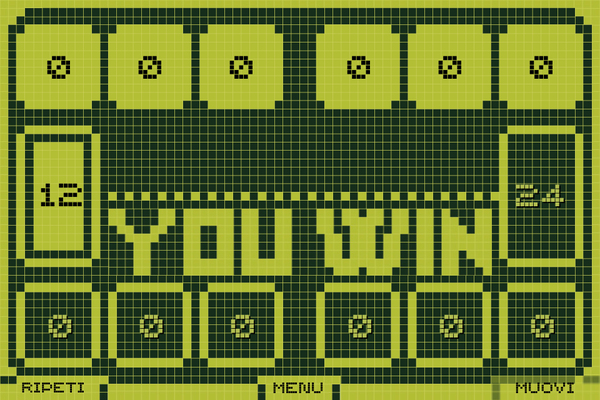
\includegraphics[width=0.3\columnwidth]{bantumi} % Example image
\end{center}
\vspace{0.8in}\LARGE{\hmwkAuthorName}\\
\Large\vspace{1in}{\hmwkYear}\\
\vspace{0.3in}
}

\author{}
\date{}

%----------------------------------------------------------------------------------------

\begin{document}

\maketitle
\newpage
\tableofcontents
\newpage


\section{Introduction}

De par sa simplicit\'e, le jeu de Bantumi est un bon candidat pour le d\'eveleppement d'une version informatis\'ee. Contrairement au jeu d'\'echecs et plus encore au jeu de go, l'arbre de recherche est relativement restreint. \`A chaque tour, le nombre de coups possible est au maximum de 6. De plus, l'\'evaluation par l'ordinateur de la force d'une position de jeu est tr\`es simple puisqu'il suffit de faire la diff\'erence entre le score d'un joueur et le score du joueur adverse. Mon impl\'ementation tentera de rester aussi simple sans sacrifier la jouabilit\'e.

\section{Choix des structures de donn\'{e}es et conventions de repr\'esentation}

Chacun des \'etats du jeu peut \^etre modelis\'e par l'ordinateur sous la forme d'une structure contenant un tableau  pour repr\'esenter l'\'etat du plateau et d'une enumeration pour representer le joueur actif.

\cscript{struct}{Structure repr\'esentant l'\'etat du jeu}

Chacun des 14 bols du jeu sera repr\'esent\'e par un \'element d'un tableau \`a deux dimensions 2x7. L'avantage d'un tel tableau est qu'il pourra \^etre adress\'e suivant les circonstances comme un tableau unidimensionnel de taille 14 ou comme deux tableaux de taille 7 qui representeront chacun le cot\'e d'un des joueurs. 

\begin{center}
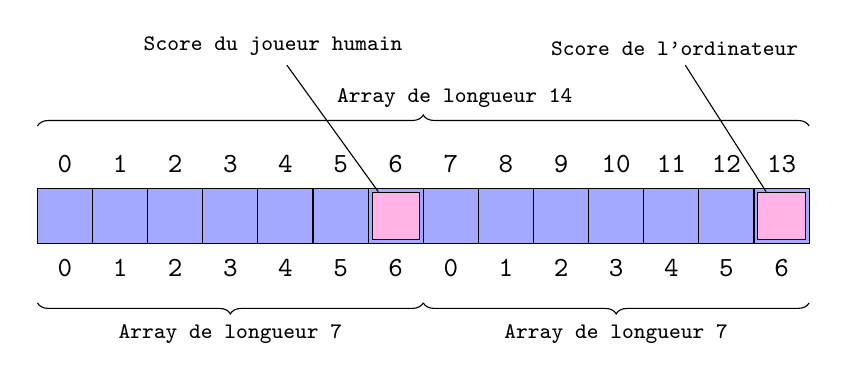
\begin{tikzpicture}[font=\ttfamily,
array/.style={matrix of nodes,nodes={draw, minimum size=7mm, fill=myblue},column sep=-\pgflinewidth, row sep=0.5mm, nodes in empty cells,
row 1/.style={nodes={draw=none, fill=none, minimum size=5mm}},
row 3/.style={nodes={draw=none, fill=none, minimum size=5mm}}}
]

\matrix[array] (array) {
0 & 1 & 2 & 3 & 4 & 5 & 6 & 7 & 8 & 9 & 10 & 11 & 12 & 13\\
  &   &   &   &   &   &   &   &   &  &  &  &  & \\
0 & 1 & 2 & 3 & 4 & 5 & 6 & 0 & 1 & 2 & 3 & 4 & 5 & 6\\};

\node[draw, fill=mypink, minimum size=6mm] at (array-2-7) (mancala0) {};
\node[draw, fill=mypink, minimum size=6mm] at (array-2-14) (mancala1) {};


\begin{scope}[on background layer]
\fill[white!10] (array-1-1.north west) rectangle (array-1-1.south east);
\end{scope}


\draw (array-1-1.north)--++(110:0mm) node [above] (first) {};

\draw [decorate,decoration={brace,amplitude=4pt,raise=4pt},yshift=0pt]
(-4.9,1.0) -- (4.9,1.0) node [black,midway,xshift=0.4cm,yshift=0.5cm] {\footnotesize Array\ de\ longueur\ 14};

\draw [decorate,decoration={brace,amplitude=4pt,mirror,raise=3pt},yshift=0pt]
(0.0,-1.0) -- (4.9,-1.0) node [black,midway,xshift=0.0cm,yshift=-0.5cm] {\footnotesize Array\ de\ longueur\ 7};

\draw [decorate,decoration={brace,amplitude=4pt,mirror,raise=3pt},yshift=0pt]
(-4.9,-1.0) -- (0.0,-1.0) node [black,midway,xshift=0.0cm,yshift=-0.5cm] {\footnotesize Array\ de\ longueur\ 7};

\node [align=center, anchor=south,xshift=-0.5cm,yshift=1.0cm] at (array-2-6.north west|-first.south) (7) {\footnotesize Score du joueur humain};

\node [align=center, anchor=south,xshift=-0.3cm,yshift=1.0cm] at (array-2-13.north west|-first.south) (14) {\footnotesize Score de l'ordinateur};

\draw (7)--(mancala0);
\draw (14)--(mancala1);

\end{tikzpicture}
\end{center}

Une particularit\'e du jeu est de se jouer dans le sens antihorlogique. L'indice 0 correspondra au premier bol en partant de la gauche du joueur humain, on fait ensuite cro\^itre les indices de gauche \`a droite jusqu'\`a l'indice 6 qui correspondra au score du joueur humain. On continue ensuite sur la partie haute du jeu en faisant cro\^{i}tre les indices de la droite vers la gauche.\\

\begin{center}
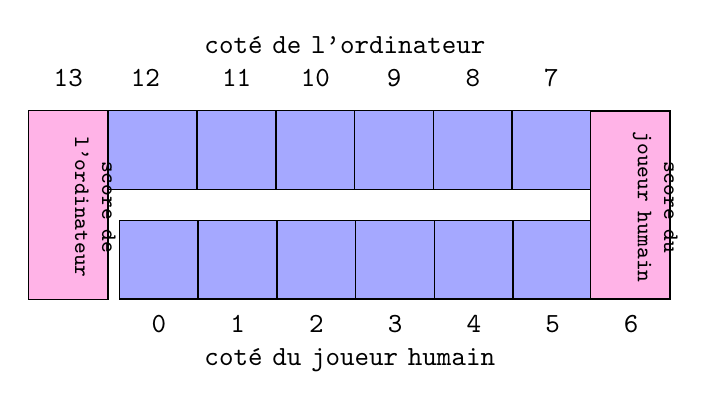
\begin{tikzpicture}[
font=\ttfamily,
every node/.style={
shape=rectangle,                                         %rounded corners,
semithick},
botarray/.style={matrix of nodes,xshift=1.7mm,nodes={draw, minimum size=10mm, fill=myblue},column sep=-\pgflinewidth, row sep=0.5mm, nodes in empty cells,
row 2/.style={nodes={draw=none, fill=none, minimum size=5mm}}},
toparray/.style={matrix of nodes,yshift=20mm,nodes={draw, minimum size=10mm, fill=myblue},column sep=-\pgflinewidth, row sep=0.5mm, nodes in empty cells,
row 1/.style={nodes={draw=none, fill=none, minimum size=5mm}},
column 1/.style={nodes={text width=10.8mm, align=center}}}
]

\matrix[botarray] (botarray) {  &  &   &   &   &   &  \\
0 & 1 & 2 & 3 & 4 & 5 & 6\\
};

\matrix[toparray] (toparray) {12 & 11 & 10 & 9 & 8 & 7 & \\
  &   &   &   &   &   &  \\
};


\node[draw, fill=mypink, minimum width=10.1mm, minimum height=23.9mm, yshift=-6.98mm, xshift=0.0mm,label={[label distance=-16.0mm,text depth=-6mm, align=center ,text width=30mm,rotate=-90]right:\footnotesize{score du \\[-0.9mm] joueur humain}}] at (toparray-2-7) (botmancala) {};

\node[draw, fill=mypink, minimum width=10.1mm, yshift=15.1mm, xshift=-61.5mm, minimum height=24.0mm, label={[label distance=1.6mm]90:13},align=center, label={[label distance=-11.0mm,text depth=-6mm, align=center ,text width=20mm,rotate=-90]right:\footnotesize{score de \\[-0.8mm] l'ordinateur}}] at (botarray-2-6) (topmancala) {};
\node[text width=5cm] at (0.25,-1.0) {cot\'e du joueur humain};
\node[text width=5cm] at (0.25,3.0) {cot\'e de l'ordinateur};
\end{tikzpicture}

\end{center}

Une autre particularit\'e dont il faudra tenir compte est la circularit\'e du plateau: si lors d'un coup on arrive \`a l'extr\'emit\'e gauche en haut du plateau, on continue la distribution dans la partie basse. Pour repr\'esenter cette circularit\'e \`a l'aide un tableau lin\'eaire, il suffira d'utiliser dans le code un indice modulo 14 qui permettra de boucler de la position 13 \`a la position 0.\\


Les joueurs seront repr\'esent\'es par une \'enumeration contenant comme membres les deux joueurs. Le joueur humain sera repr\'esent\'e par un 0 et l'ordinateur par un 1. Cela permettra d'adresser chacune des deux parties du tableau avec le nom des joueurs, pour obtenir leur score par exemple: \texttt{score = board[human][6];}

\section{D\'efinition des \'ecrans}

On peut envisager le programme comme un automate fini dont les \'ecrans repr\'esentent les \'etats, et dont les entr\'ees du joueur d\'eclenchent les transitions d'un \'etat vers un autre.\\

\begin{figure}[!ht]
  \caption{Diagramme des transitions entre les \'ecrans}
  \centering
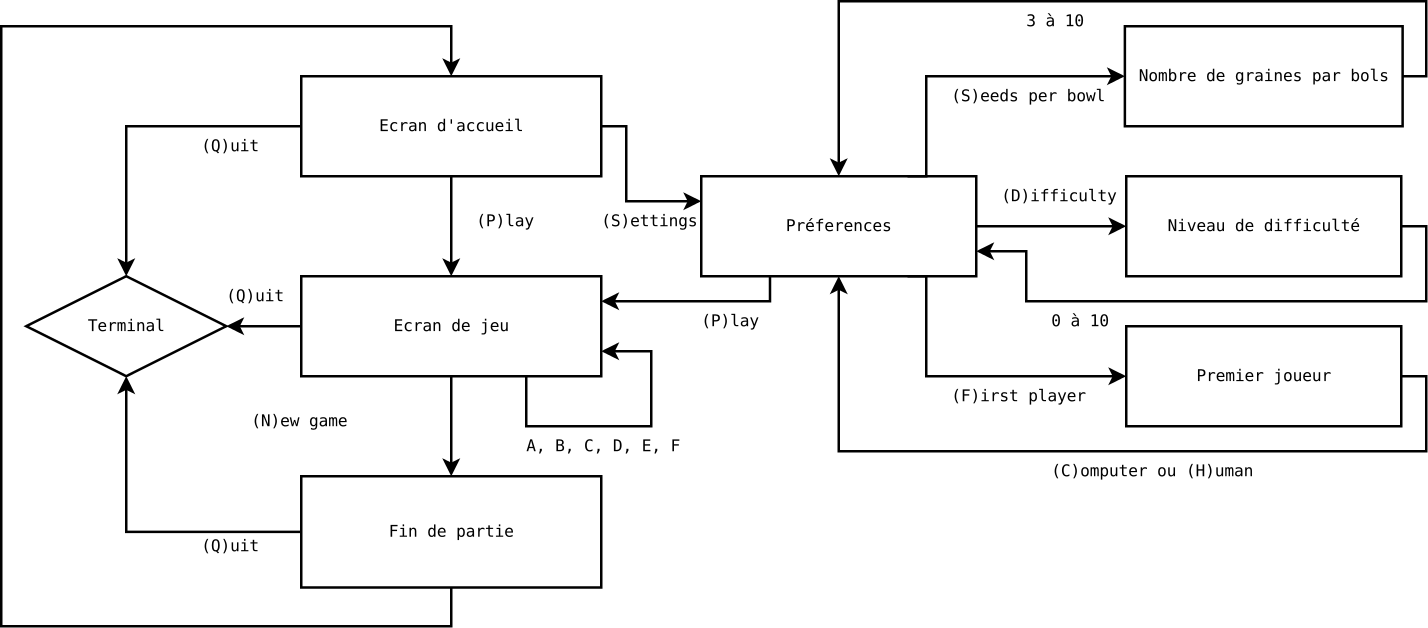
\includegraphics[width=1.0\columnwidth]{diagram.png}{} % Example image
\end{figure}

Le premier \'ecran sera l'\'ecran d'accueil. Celui ci proposera au joueur soit de commencer \`a jouer avec une configuration choisie al\'eatoirement (premier joueur, nombres de graines par emplacement, niveau de difficult\'e), soit de laisser le joueur d\'efinir manuellement ces param\`etres.\\

\cscript{welcome}{\'Ecran d'accueil}

Si le joueur d\'ecide de commencer directement \`a jouer, un \'ecran comportant une description du plateau de jeu lui sera pr\'esent\'e suivi d'une invite de commande lui demandant quel coup jouer. Apr\`es chaque coup, cet \'ecran sera mis \`a jour avec la derni\`ere configuratoin du plateau et l'indication du joueur dont c'est le tour, jusqu'\`a la victoire d'un des deux joueurs. \`A tout moment, le joueur aura aussi la possibilit\'e de quitter le jeu et de retourner vers le terminal.

\cscript{game}{\'Ecran de jeu}

Lorsque le programme aura d\'etect\'e la fin de la partie, un \'ecran affichera le score et une invite de commande proposera au joueur soit de quitter, soit de rejouer (retour \`a l'\'ecran d'accueil).

\cscript{endgame}{\'Ecran de fin de partie}

Le jeu comportera aussi des \'ecrans pour la configuration. Ceux-ci restent \`a d\'efinir.

\section{D\'ecoupe du probl\`eme en sous probl\`emes}

En plus du fichier contenant la fonction \texttt{main()}, on divisera le code en trois unit\'es fonctionnelles contenues dans trois paires de fichiers .c/.h:

\begin{enumerate}

\item[1.]
Les fichiers game.c/game.h contiendront les d\'efinitions des structures de donn\'ees repr\'esentant le plateau et les joueurs, et la fonction permettant d'effectuer un coup selon les r\`egles du jeu, une fonction d'initialisation du plateau en d\'ebut de partie, une fonction permettant de reconnaitre la fin de la partie et une fonction permettant d'obtenir le score d'un joueur.

\item[2.]
Les fichiers ui.c/ui.h (\textit{user interafce}) contiendront les fonctions qui g\`ereront les entr\'ees du joueur humain et l'affichage des differents \'ecrans d\'efinis dans la section pr\'ec\'edente.
La fonction principlale sera la gestion appel\'ee par \texttt{main()} au commencement du jeu. Cette fonction procedera \'a des \texttt{scanf()} pour lire les choix du joueur humain et lancera les fonctions correspondantes, ou invitera le joueur \`a rep\'eter son choix en cas d'entr\'ee invalide. 

\item[3.]
Les fichiers strategy.c/strategy.h contiendront les fonctions utilis\'ees par l'ordinateur pour d\'efinir sa strat\'egie de jeu. Ces fonctions restent \`a d\'efinir.

\end{enumerate}
%----------------------------------------------------------------------------
\section{Conclusion}

En plus du programme lui-meme, ce projet a \'et\'e pour moi l'occasion d'apprendre different outils comme github, Latex, Makefile.



\bigskip
\bigskip

\renewcommand\refname{Ref\'erences}

\begin{thebibliography}{9}
\medskip
\bibitem{latexcompanion} 
Michel Goossens, Frank Mittelbach, and Alexander Samarin. 
\textit{The \LaTeX\ Companion}. 
Addison-Wesley, Reading, Massachusetts, 1993.
 
\bibitem{einstein} 
Albert Einstein. 
\textit{Zur Elektrodynamik bewegter K{\"o}rper}. (German) 
[\textit{On the electrodynamics of moving bodies}]. 
Annalen der Physik, 322(10):891–921, 1905.
 
\bibitem{knuthwebsite} 
Knuth: Computers and Typesetting,
\\\texttt{http://www-cs-faculty.stanford.edu/\~{}uno/abcde.html}
\end{thebibliography}

\bibitem{minimax} 
Minimax search and alpha-beta pruning
\\\texttt{https://www.cs.cornell.edu/courses/cs312/2002sp/lectures/rec21.htm}
\end{thebibliography}

\bibliography{biblio}{}
\bibliographystyle{unsrt}
\end{document}
